% !TeX program = pdflatex
% ============================================================
% CiboAmico — Final ISPW report (Tor Vergata, A.Y. 2025/2026)
% Prof. Davide Falessi & Prof. Guglielmo De Angelis
% ENGLISH version
% ============================================================
\documentclass[12pt,a4paper,oneside]{report}

% --- Language and encoding ---
\usepackage[english]{babel}
\usepackage[utf8]{inputenc}
\usepackage[T1]{fontenc}
\usepackage{microtype}

% --- Geometria e tipografia ---
\usepackage[margin=2.5cm]{geometry}
\usepackage{setspace}
\onehalfspacing

% --- Images, tables ---
\usepackage{graphicx}
\usepackage{booktabs}
\usepackage{colortbl}
\usepackage{float}
\usepackage{pdflscape}
\usepackage{array}
\usepackage{multirow}
\usepackage{caption}
\captionsetup{font=small,labelfont=bf}

% --- Lists and symbols ---
\usepackage{enumitem}
\usepackage{csquotes}
\usepackage{amsmath,amssymb}
\usepackage{xcolor}

% --- UML / diagrams ---
\usepackage{tikz}
\usetikzlibrary{shapes,shapes.geometric,positioning,arrows.meta}

% --- Java code ---
\usepackage{listings}
\definecolor{codegray}{RGB}{245,245,245}
\definecolor{codekeyword}{RGB}{0,0,204}
\definecolor{codecomment}{RGB}{0,128,0}
\definecolor{codestring}{RGB}{163,21,21}
\lstset{
    language=Java,
    basicstyle=\ttfamily\footnotesize,
    keywordstyle=\color{codekeyword},
    commentstyle=\color{codecomment},
    stringstyle=\color{codestring},
    backgroundcolor=\color{codegray},
    frame=single,
    breaklines=true,
    columns=fullflexible,
    captionpos=b
}

% --- Links ---
\usepackage{hyperref}
\hypersetup{
    colorlinks=true,
    linkcolor=black,
    urlcolor=blue,
    citecolor=black
}

% ============================================================
\begin{document}

% --- Title page ---
\begin{titlepage}
    \centering
    \large
    \textbf{UNIVERSITÀ DEGLI STUDI DI ROMA ``TOR VERGATA''} \\[0.3cm]
    \large Macroarea di Ingegneria \\[1.2cm]

    \scshape\Large Corso di Laurea in Ingegneria Informatica \\[0.3cm]
    \large Ingegneria del Software e Progettazione Web (ISPW) \\[1.5cm]

    \rule{\linewidth}{0.4mm} \\[0.4cm]
    {\huge\bfseries CiboAmico} \\[0.3cm]
    \large\itshape Platform for managing food at home, reducing waste and optimising the shopping experience \\
    \rule{\linewidth}{0.4mm} \\[1.5cm]

    \begin{minipage}{0.5\textwidth}
        \begin{flushleft} \large
            \emph{Supervisors:} \\
            Prof. Davide Falessi \\
            Prof. Guglielmo De Angelis
        \end{flushleft}
    \end{minipage}
    \hfill
    \begin{minipage}{0.42\textwidth}
        \begin{flushright} \large
            \emph{Author:} \\
            \textbf{Michele \textsc{Damiano}} \\
            Student ID: 0324516 \\
            \href{mailto:michele.damiano@students.uniroma2.eu}{\small michele.damiano@students.uniroma2.eu}
        \end{flushright}
    \end{minipage} \\[2.5cm]

    \vfill
    {\large Academic Year 2025/2026} \\[0.2cm]
    {\large Submission date: \today}
\end{titlepage}

% --- Table of contents ---
\tableofcontents
\newpage

% ============================================================
% CHAPTERS
% ============================================================
% ============================================================
% CHAPTER 1 — SOFTWARE REQUIREMENTS SPECIFICATION (SRS)
% ============================================================
\chapter{Software Requirements Specification}
\label{cap:srs}

% ------------------------------------------------------------
\section{Introduction}
\label{sec:intro}

\subsection{Purpose of the document}
\label{subsec:scopo}

This document defines the software requirements of \textbf{CiboAmico}, the final project of the ISPW course (University of Rome ``Tor Vergata'', A.Y.\ 2025/2026, Prof. Davide Falessi, Prof. Guglielmo De Angelis).

The purpose is to state what the system shall do in a clear and verifiable way, leaving room for design and testing. The document serves both developers, who must keep the Boundary-Control-Entity (BCE) architecture, and the evaluators, who compare the functional flows against the initial requests.

\subsection{System overview}
\label{subsec:panoramica}

CiboAmico is a desktop JavaFX application that helps manage food at home, avoid waste and optimise the shopping experience by connecting the user with local vendors. The system follows the Boundary-Control-Entity (BCE) pattern and involves four actors: Customer, Vendor, Nutritionist and Administrator. Two external systems are reached through an Adapter: OpenFoodFacts (reading nutritional data from the barcode) and JakartaMail (sending notifications). Persistence is interchangeable at runtime between a \textit{Demo} (in-memory) and a \textit{Full} (MySQL via JDBC) mode.

The system has three functional areas:
\begin{itemize}
    \item \textbf{Pantry}: the Customer keeps track of the food at home, sees the expiry dates and is warned before the food goes bad;
    \item \textbf{Recipes}: the system proposes recipes compatible with the available ingredients, substituting the missing ones;
    \item \textbf{Marketplace}: the Vendors publish products, the Customers place direct orders (one buyer, one vendor) and the Administrator approves vendors and recipes.
\end{itemize}

\subsection{Hardware and software requirements}
\label{subsec:requisiti_hw_sw}

The application is cross-platform thanks to the JVM.

\textbf{Software requirements:}
\begin{itemize}
    \item Java 17+
    \item JavaFX 17+ (for the desktop interface)
    \item Maven 3.9+ (build tool)
    \item MySQL Server 8.0+ (\textit{Full} mode, via JDBC)
    \item Draw.io (for creating the UML diagrams)
    \item IDE: IntelliJ IDEA (with EclEmma for coverage) or Eclipse
\end{itemize}

\textbf{Hardware requirements:}
\begin{itemize}
    \item CPU: Dual-Core 2.0~GHz 64-bit
    \item RAM: 2~GB (4~GB recommended in \textit{Full} mode with a local MySQL server)
    \item Disk space: 1~GB
    \item Screen: $1024\times768$
    \item Operating system: Windows, macOS, Linux (compatible with Java 17+)
\end{itemize}

\subsection{Related systems}
\label{subsec:relazionati}

Two existing systems cover only in part what CiboAmico does.

\textbf{System 1: Too Good To Go}

\textbf{Pros:}
\begin{itemize}
    \item Wide network of partners with geolocated offers in real time.
    \item Actively reduces commercial waste by offering food at reduced prices.
\end{itemize}

\textbf{Cons:}
\begin{itemize}
    \item It does not track the home pantry: after the purchase it does not help manage the expiry dates.
    \item The purchase is a surprise \emph{Magic Box}: the user does not choose the single products nor plan recipes or diets.
\end{itemize}

\textbf{System 2: SuperCook}

\textbf{Pros:}
\begin{itemize}
    \item Powerful matching: it quickly finds many recipes from the inserted ingredients.
    \item Large database with filters by dish type and intolerances.
\end{itemize}

\textbf{Cons:}
\begin{itemize}
    \item It has no integrated purchase channel: the user must buy the missing ingredients by themselves.
    \item It does not automatically substitute the ingredients, excluding recipes that would be possible with small variations.
\end{itemize}

CiboAmico aims to combine pantry tracking, recipe generation with substitutions and direct purchase from local producers in a single platform, providing features dedicated to customers, vendors, nutritionists and administrators while keeping a modular and extensible architecture.

% ------------------------------------------------------------
\section{User Stories}
\label{sec:user_stories}

\begin{enumerate}
    \item \textbf{US-1}: As a Customer, I want to purchase products from verified local vendors, so that I can support nearby businesses and receive my items faster.
    \item \textbf{US-2}: As a Customer, I want to apply a promotional voucher code during checkout, so that I can reduce the total cost of my order and save money.
    \item \textbf{US-3}: As a Customer, I want to pay for my order securely using my credit card, so that I can complete my purchase immediately without handling physical cash.
\end{enumerate}

% ------------------------------------------------------------
\section{Functional Requirements}
\label{sec:requisiti_funzionali}

\begin{enumerate}
    \item \textbf{FR-1}: The system shall display the catalog of the products published by approved vendors, with price and available quantity.
    \item \textbf{FR-2}: The system shall apply a promotional voucher to the current order when the code is valid and belongs to the vendor of the selected product.
    \item \textbf{FR-3}: The system shall register a purchase order by associating the customer with the vendor and decreasing the product stock by the ordered quantity.
\end{enumerate}

\subsection{Glossary of Domain Terms}
\begin{description}
    \item[\textbf{Catalog}]: set of products published by approved vendors and made available for purchase in the marketplace.
    \item[\textbf{Promotional voucher}]: discount code associated with a specific vendor, valid within a time window and applicable to an order of that vendor.
    \item[\textbf{Direct order}]: transaction that associates a single buying customer with a single vendor, without passing through a shared cart or intermediaries.
    \item[\textbf{Product availability}]: quantity of a product currently sellable, which can never be negative and is updated after every purchase.
\end{description}

% ------------------------------------------------------------
\section{Use Cases}
\label{sec:use_cases}

\subsection{Use case diagram}
\label{subsec:uc_diagramma}

\begin{figure}[H]
    \centering
    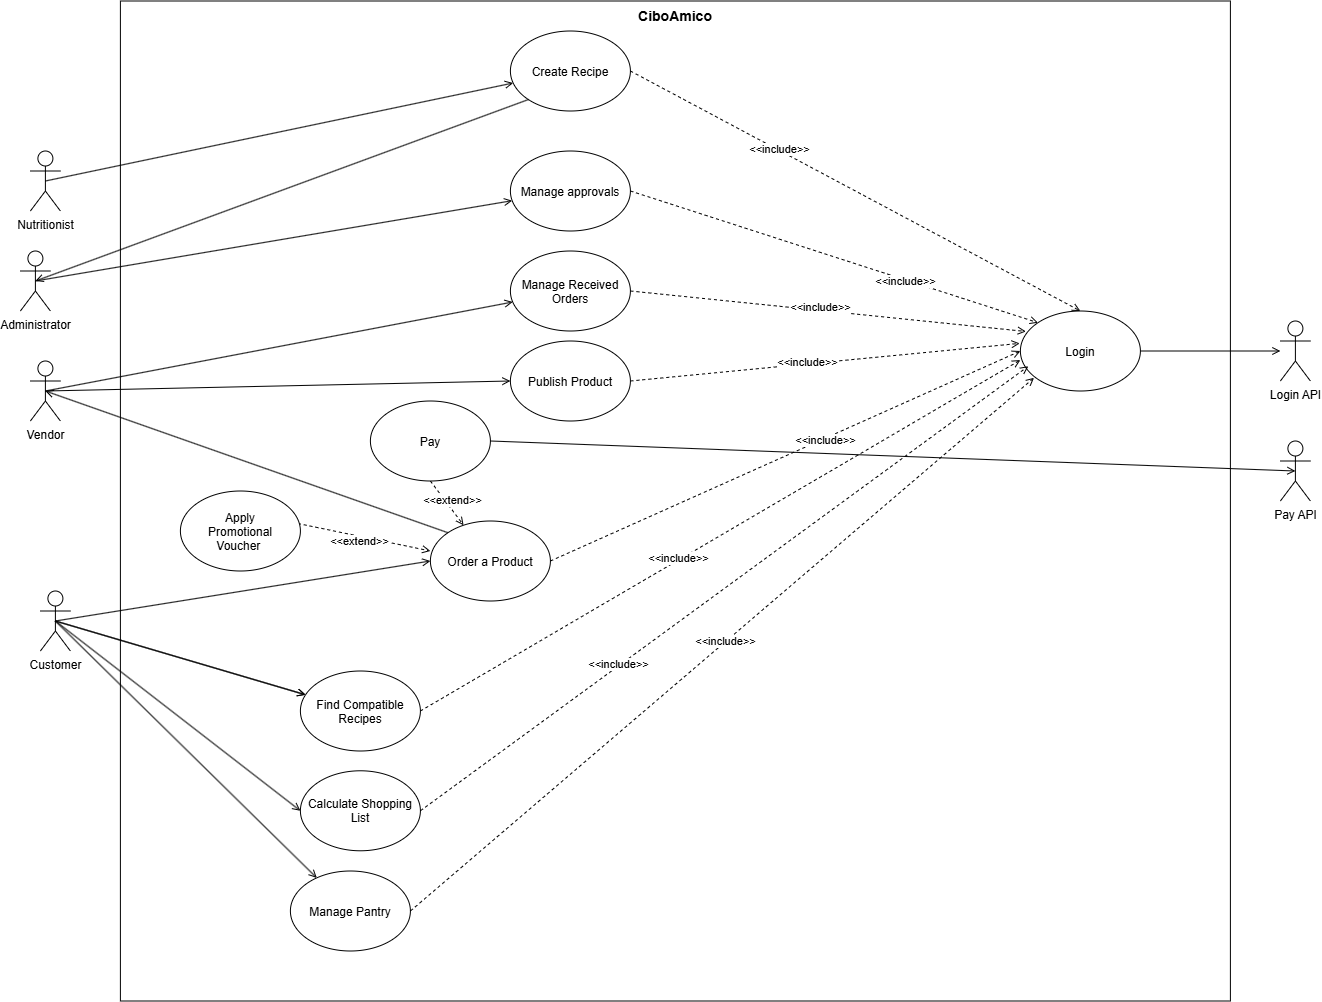
\includegraphics[width=0.95\textwidth]{figures/usecase_diagram_hr.png}
    \label{fig:usecase_diagram}
\end{figure}

\subsection{Internal Steps}
\label{subsec:uc_internal_steps}
\clearpage

\subsubsection{Order a Product}
\label{u:uc04}

\textbf{Main Flow:}
\begin{enumerate}
    \item The customer accesses the marketplace via Login.
    \item The system displays the available products with price and remaining stock.
    \item The customer selects a product from the catalog and starts the checkout.
    \item The system loads the selected product into the current order and computes the total amount.
    \item The customer confirms the purchase.
    \item The system requests the authorization for the debit of the computed amount from the Payment Service.
    \item The system registers the order in the ``CREATED'' state, decreases the remaining stock of the product and notifies the vendor.
\end{enumerate}

\textbf{Preconditions:} the customer is authenticated; at least one product is available in the catalog.

\textbf{Alternative Flow (Extensions):}
\begin{itemize}
    \item \textbf{3a. Product No Longer Available:} the selected product is not present in the catalog anymore; the system displays an error message.
    \item \textbf{4a. Promotional Voucher Request:} the customer requests to apply a promotional voucher to the current order; the system validates the temporal validity of the voucher and its association with the vendor of the selected product, recalculates the total amount applying the discount and resumes from step 5.
    \item \textbf{6a. Payment Rejected:} the Payment Service returns a negative outcome; the system cancels the current order and displays a failure message, returning the flow to step 4.
\end{itemize}

% CHAPTER 2 — STORYBOARDS
\chapter{Storyboards}
\label{cap:storyboards}

\section{Authentication and Personal Area}

\subsection{Login}
The login screen allows the user to authenticate by inserting their credentials (email and password).
\begin{figure}[H]
    \centering
    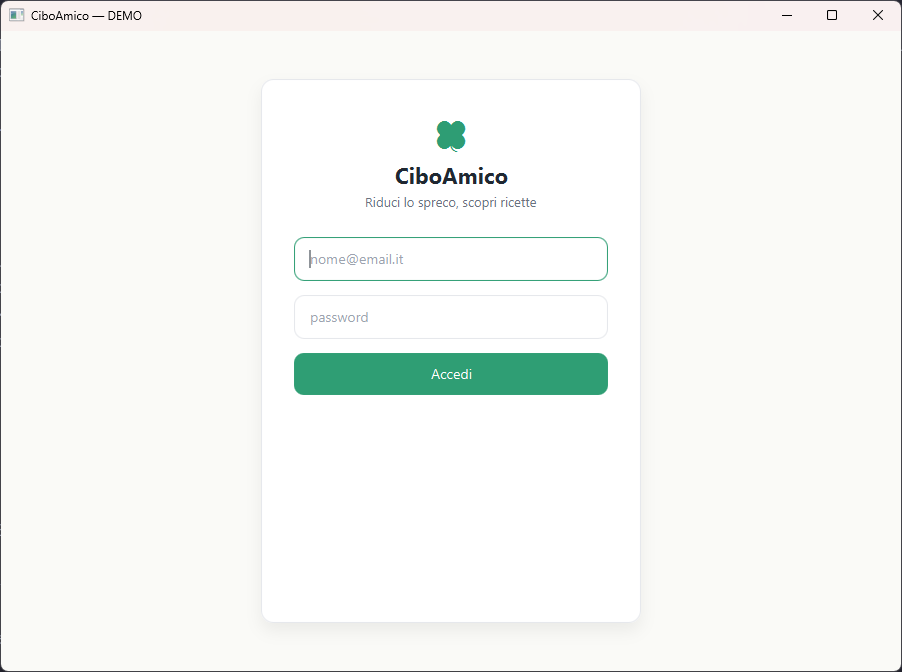
\includegraphics[width=0.8\textwidth]{figures/schermata-login.png}
    \caption{Authentication screen of the system.}
    \label{fig:sb_login}
\end{figure}

\subsection{Home (Customer)}
Once authentication is completed, the Customer reaches the main dashboard (Home). From here they can access the application features: Recipes, Inventory, Shopping List and Marketplace (UC-04 Order a Product).
\begin{figure}[H]
    \centering
    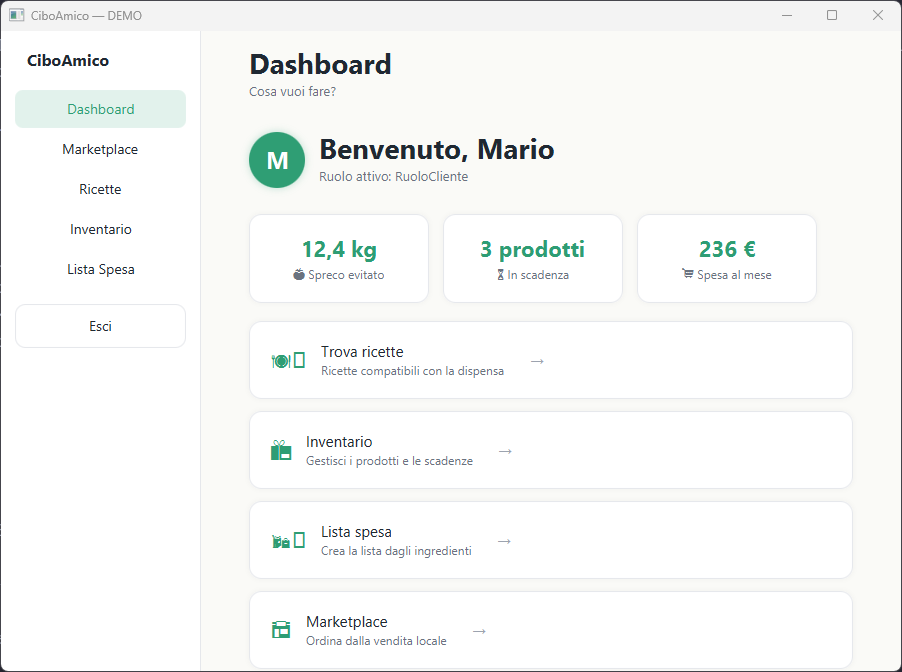
\includegraphics[width=0.8\textwidth]{figures/schermata-home.png}
    \caption{Main dashboard: access to the application features.}
    \label{fig:sb_home}
\end{figure}

\section{Purchases and Marketplace (UC-04 Order a Product)}

\subsection{Marketplace (Product Catalog)}
The area dedicated to direct purchase shows the catalog of local vendor products. The side panel allows the user to select a product to order and, optionally, a promotional voucher.
\begin{figure}[H]
    \centering
    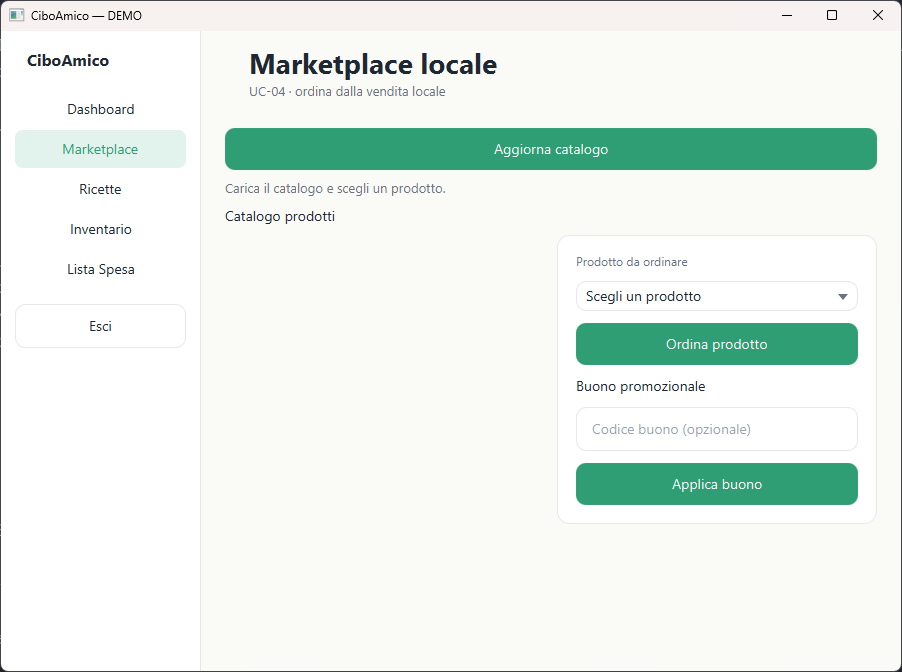
\includegraphics[width=0.8\textwidth]{figures/schermata-marketplace.png}
    \caption{Marketplace: local product catalog and purchase panel.}
    \label{fig:sb_marketplace}
\end{figure}

\subsection{Order a Product}
After selecting a product from the catalog and loading the list (button \emph{Refresh catalog}), the Customer chooses the product in the \emph{Product to order} panel. If they insert a voucher code and press \emph{Apply voucher}, the system validates the voucher and recalculates the total by applying the discount (extension \emph{Order a Product}); by pressing \emph{Order product} the flow proceeds.
\begin{figure}[H]
    \centering
    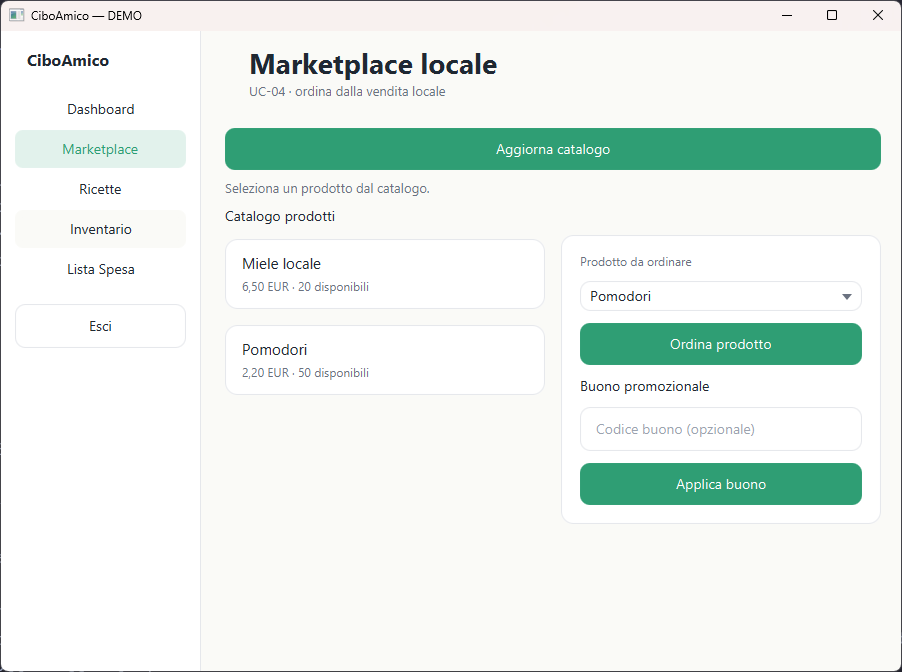
\includegraphics[width=0.8\textwidth]{figures/schermata-ordine.png}
    \caption{Purchase screen with the selected product and the promotional voucher field.}
    \label{fig:sb_ordine}
\end{figure}

\subsection{Payment (step 6)}
Once the order is confirmed, the interface moves to the payment screen: the user inserts the card data (number, holder, expiry date and CVV) and authorizes the debit; the outcome is shown inline in the same view, as required by extension \textbf{6a} (rejected payment) of the use case.
\begin{figure}[H]
    \centering
    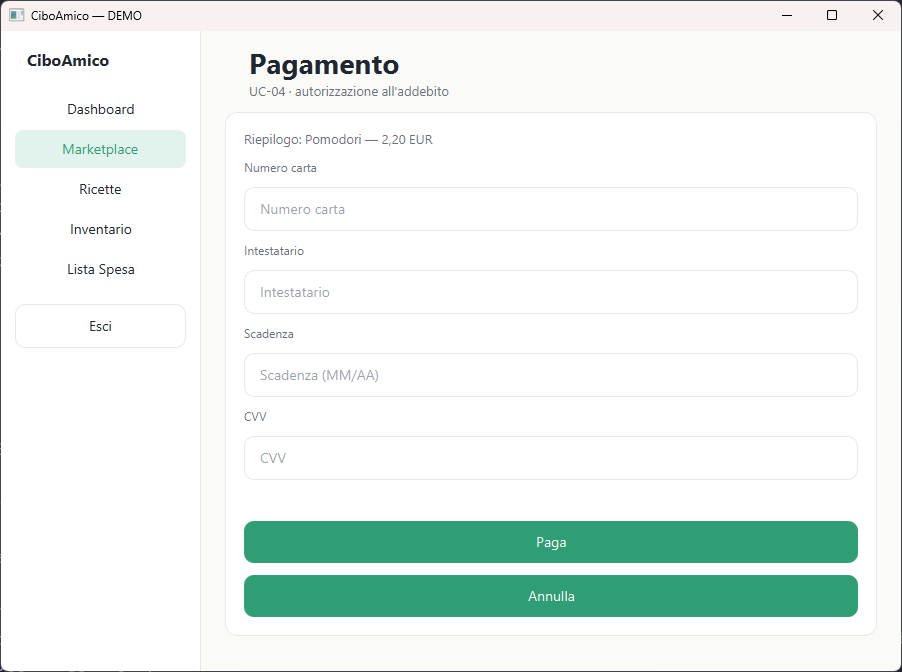
\includegraphics[width=0.8\textwidth]{figures/schermata-payment.png}
    \caption{Payment screen (card data and debit authorization).}
    \label{fig:sb_payment}
\end{figure}

\chapter{Design}
\label{cap:design}

\section{Class Diagram}
\label{sec:class_diagram}

\subsection{VOPC (Analysis)}
\label{subsec:vopc}

\begin{figure}[H]
    \centering
    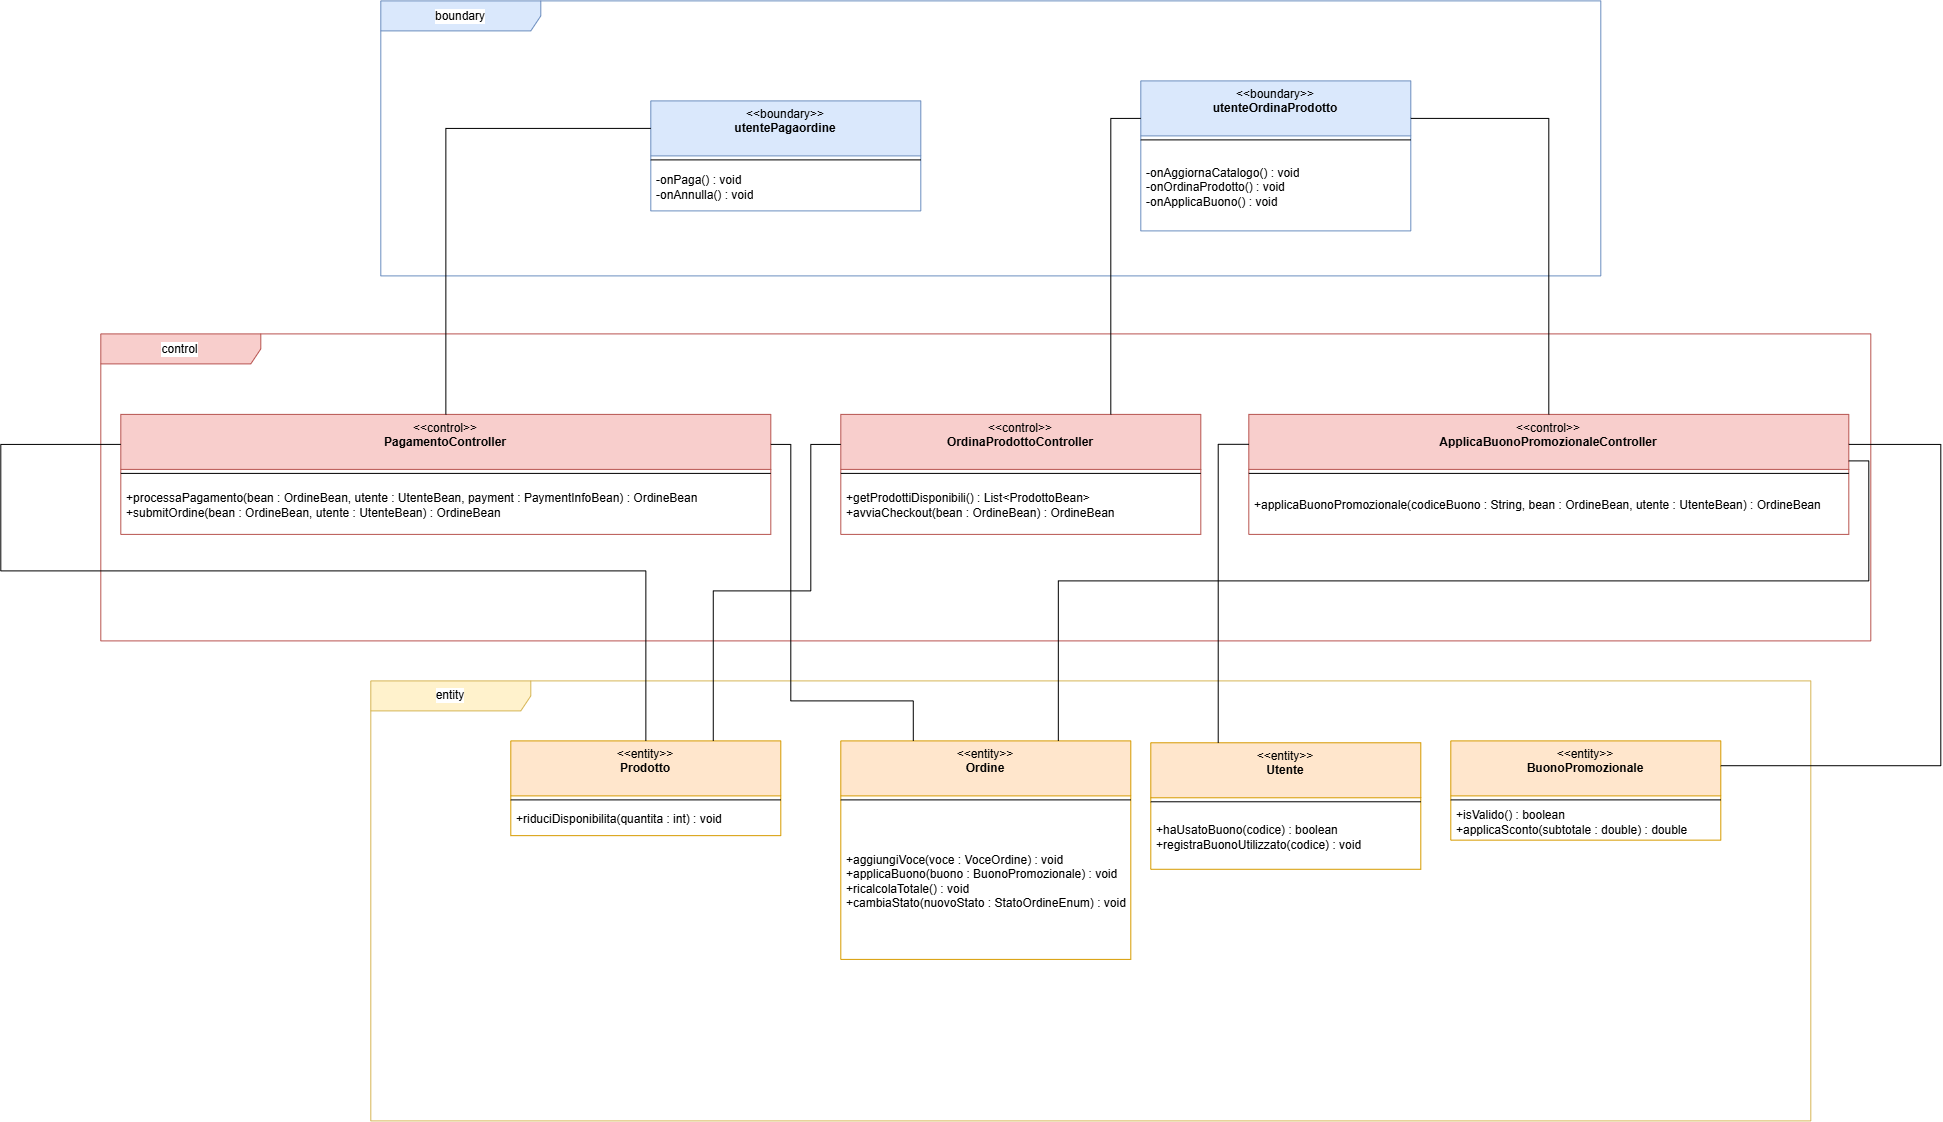
\includegraphics[width=\textwidth]{figures/vopc_uc04.png}
    \caption{VOPC of UC-04: Boundary (View), graphic controller, Facade, application controllers and Entity.}
    \label{fig:vopc}
\end{figure}

\subsection{Design Patterns}
\label{subsec:design_patterns}
The design level introduces the interfaces, the Java types, the exceptions and
the GoF patterns to manage extensibility and dynamic persistence (NFR-01). For
each pattern, the schema and a short description of its application are shown
in order.

\subsubsection*{Abstract Factory Pattern -- Persistence Layer}
\begin{figure}[H]
    \centering
    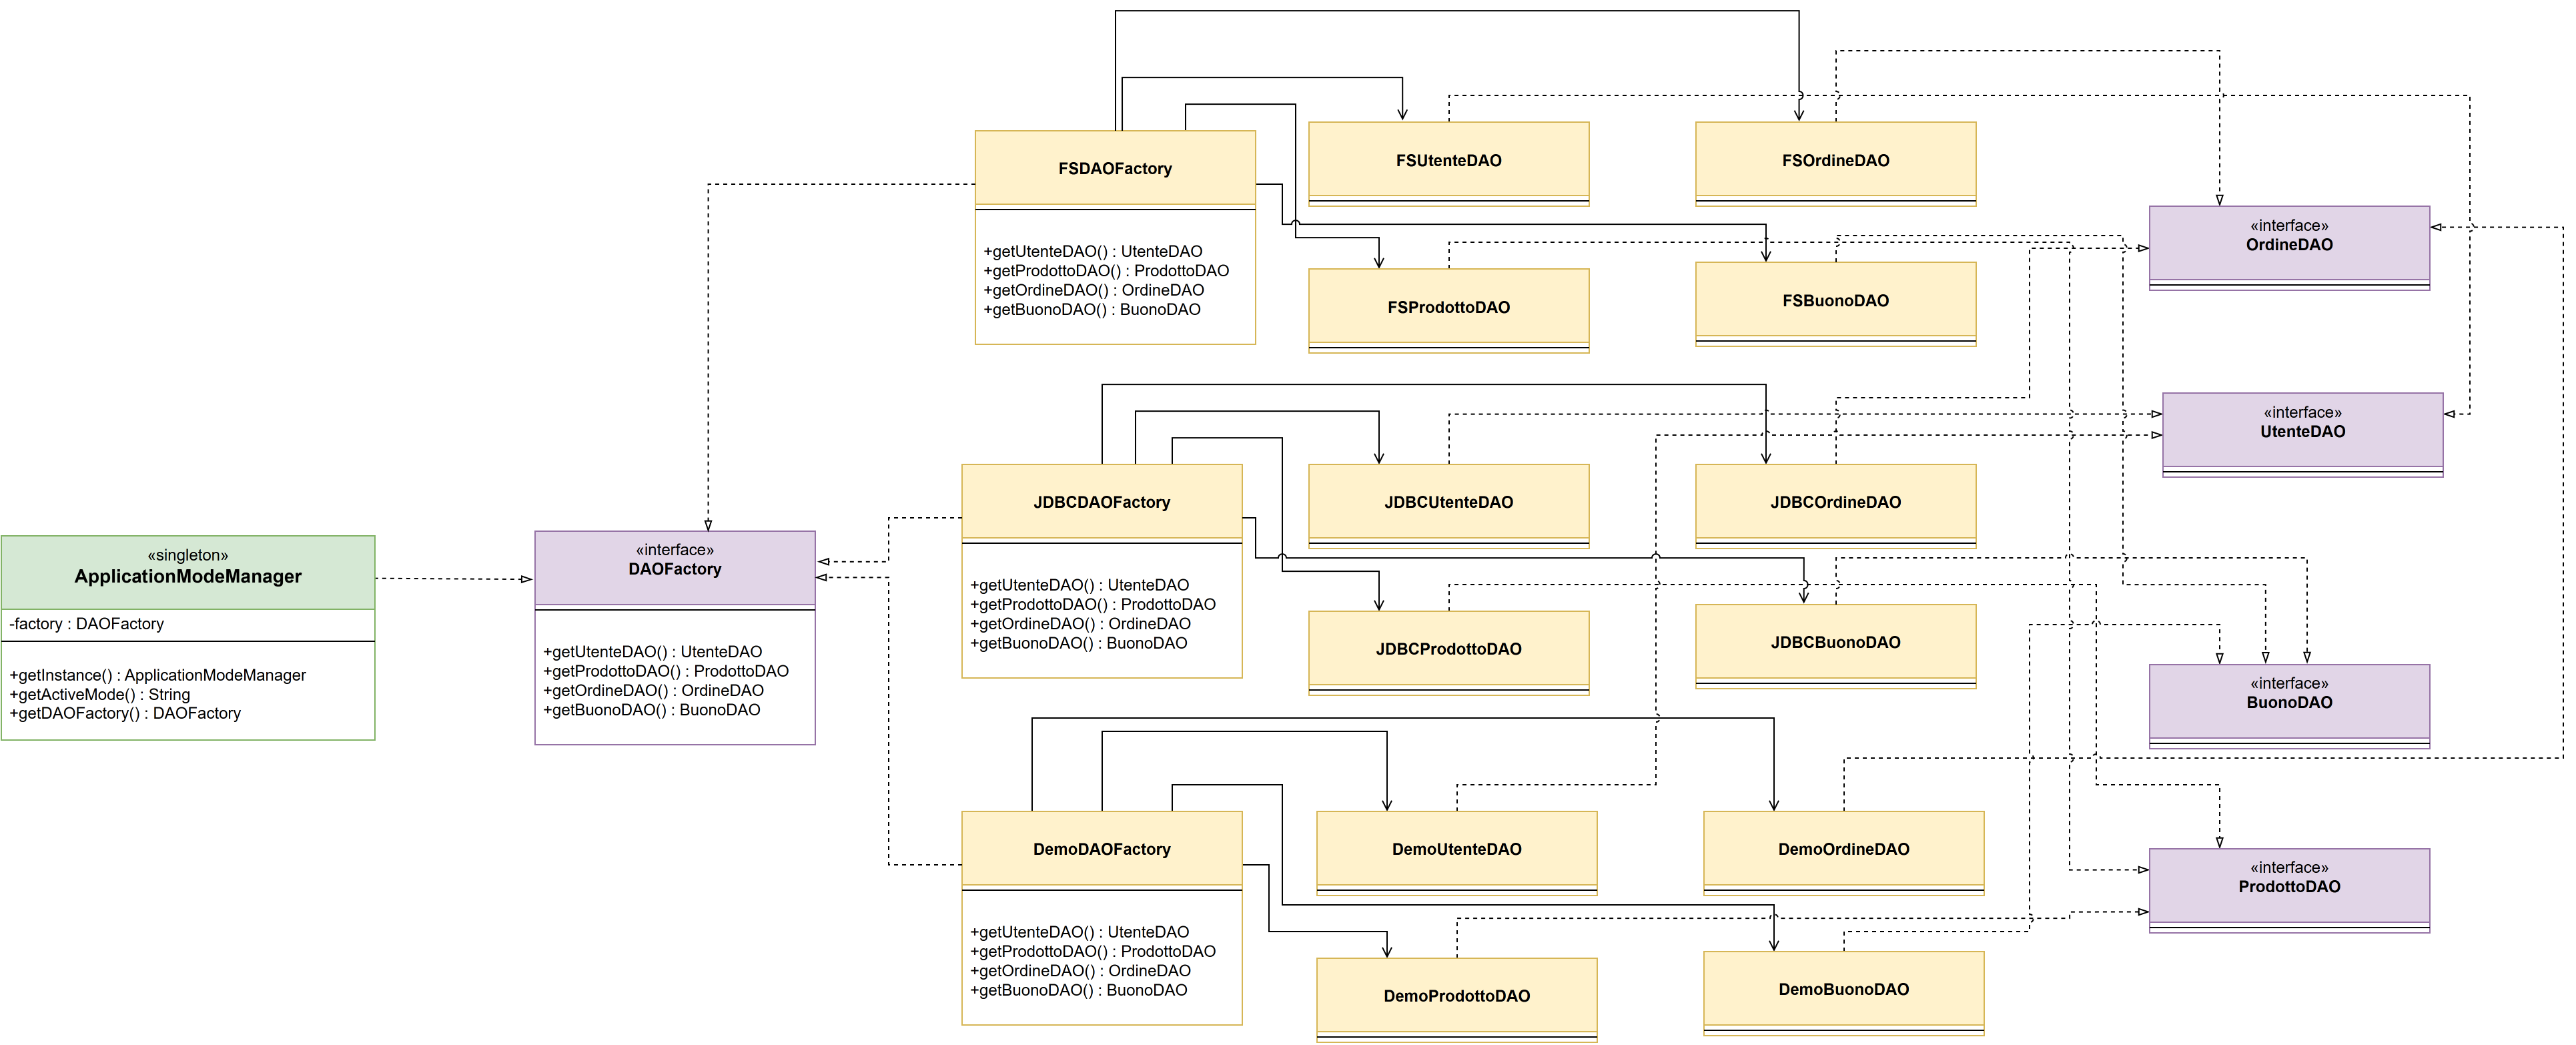
\includegraphics[width=0.85\textwidth]{figures/dl_factory_hr.png}
    \caption{Abstract Factory of the persistence: DAO interfaces, concrete DAOs and factories.}
    \label{fig:dl_factory}
\end{figure}
The persistence layer is managed through the \textbf{Abstract Factory} pattern
in order to guarantee flexibility in configuring the execution environment. The
\texttt{DAOFactory} interface defines the contract for creating the different
Data Access Objects, such as \texttt{getOrdineDAO()} and \texttt{getProdottoDAO()}.
According to the \texttt{persistence\_type} property, the concrete factories
(\texttt{JDBCDAOFactory}, \texttt{FSDAOFactory}, \texttt{DemoDAOFactory})
instantiate the appropriate storage implementation. This allows the system to
switch seamlessly between a database-based, file-system-based or in-memory
persistence without requiring any change in the client code.

\subsubsection*{Observer Pattern -- Notification System}
\begin{figure}[H]
    \centering
    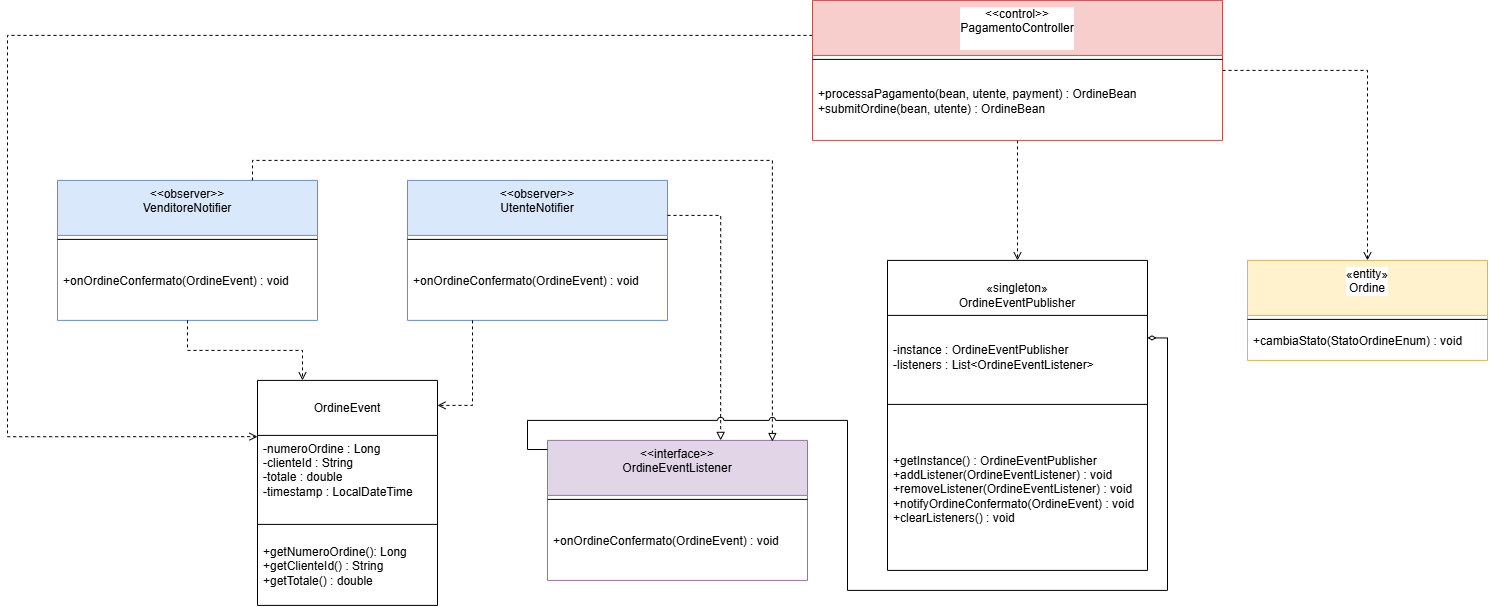
\includegraphics[width=0.55\textwidth]{figures/dl_observer_hr.png}
    \caption{Observer of the order confirmation: singleton publisher and DTO.}
    \label{fig:dl_observer}
\end{figure}
The \textbf{Observer} pattern has been implemented with the aim of decoupling
the order processing from the notification management logic. The
\texttt{OrdineEventPublisher} class acts as a \emph{Subject} implemented through
the \textbf{Singleton} pattern, managing a list (\texttt{List}) of observers of
type \texttt{OrdineEventListener}. Upon the correct submission and confirmation
of the order, the publisher invokes the \texttt{onOrdineConfermato()} method on
all the registered listeners (buyer and vendor), passing the read-only DTO
\texttt{OrdineEvent}, never the domain entity. This architecture guarantees
loose coupling between the main business logic and its side effects, strictly
respecting the \emph{Open/Closed Principle}.

The notification is emitted by the application subsystem (the control that
confirms the order) through the publisher, and not by the \texttt{Ordine}
entity: the domain entity thus remains \emph{decoupled} from the presentation
layer and from the notification mechanism. The variant is the
\emph{publish-subscribe}/event-driven one of the Observer: the coupling between
\texttt{OrdineEventPublisher} (Subject) and the observers is abstract (only
\texttt{OrdineEventListener}), the notification is a broadcast to all the
registered listeners and the exchanged data is the read-only DTO
\texttt{OrdineEvent}, never the entity.

\subsubsection*{Singleton Pattern -- Sessions and Mode}
\begin{figure}[H]
    \centering
    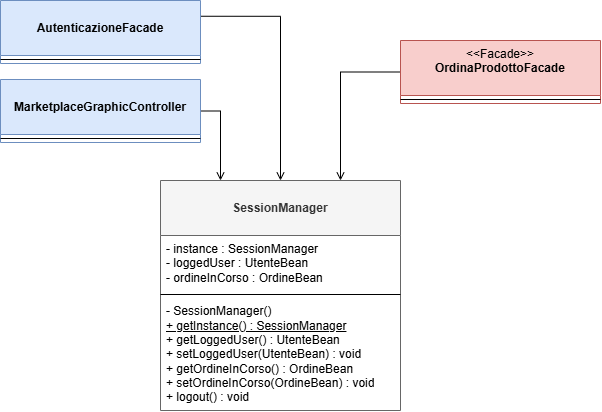
\includegraphics[width=0.55\textwidth]{figures/dl_singleton_hr.png}
    \caption{Singleton of the session and of the mode.}
    \label{fig:dl_singleton}
\end{figure}
\texttt{SessionManager} (user session) and \texttt{ApplicationModeManager}
(application mode) adopt a classic singleton with \emph{lazy
initialization} (\texttt{if (instance == null) instance = new X()}) and
synchronization on \texttt{getInstance()}, in line with the reference projects:
no perceivable cost in a desktop client, no SonarCloud warning suppression.

\subsubsection*{Facade Pattern -- Checkout UC-04}
\begin{figure}[H]
    \centering
    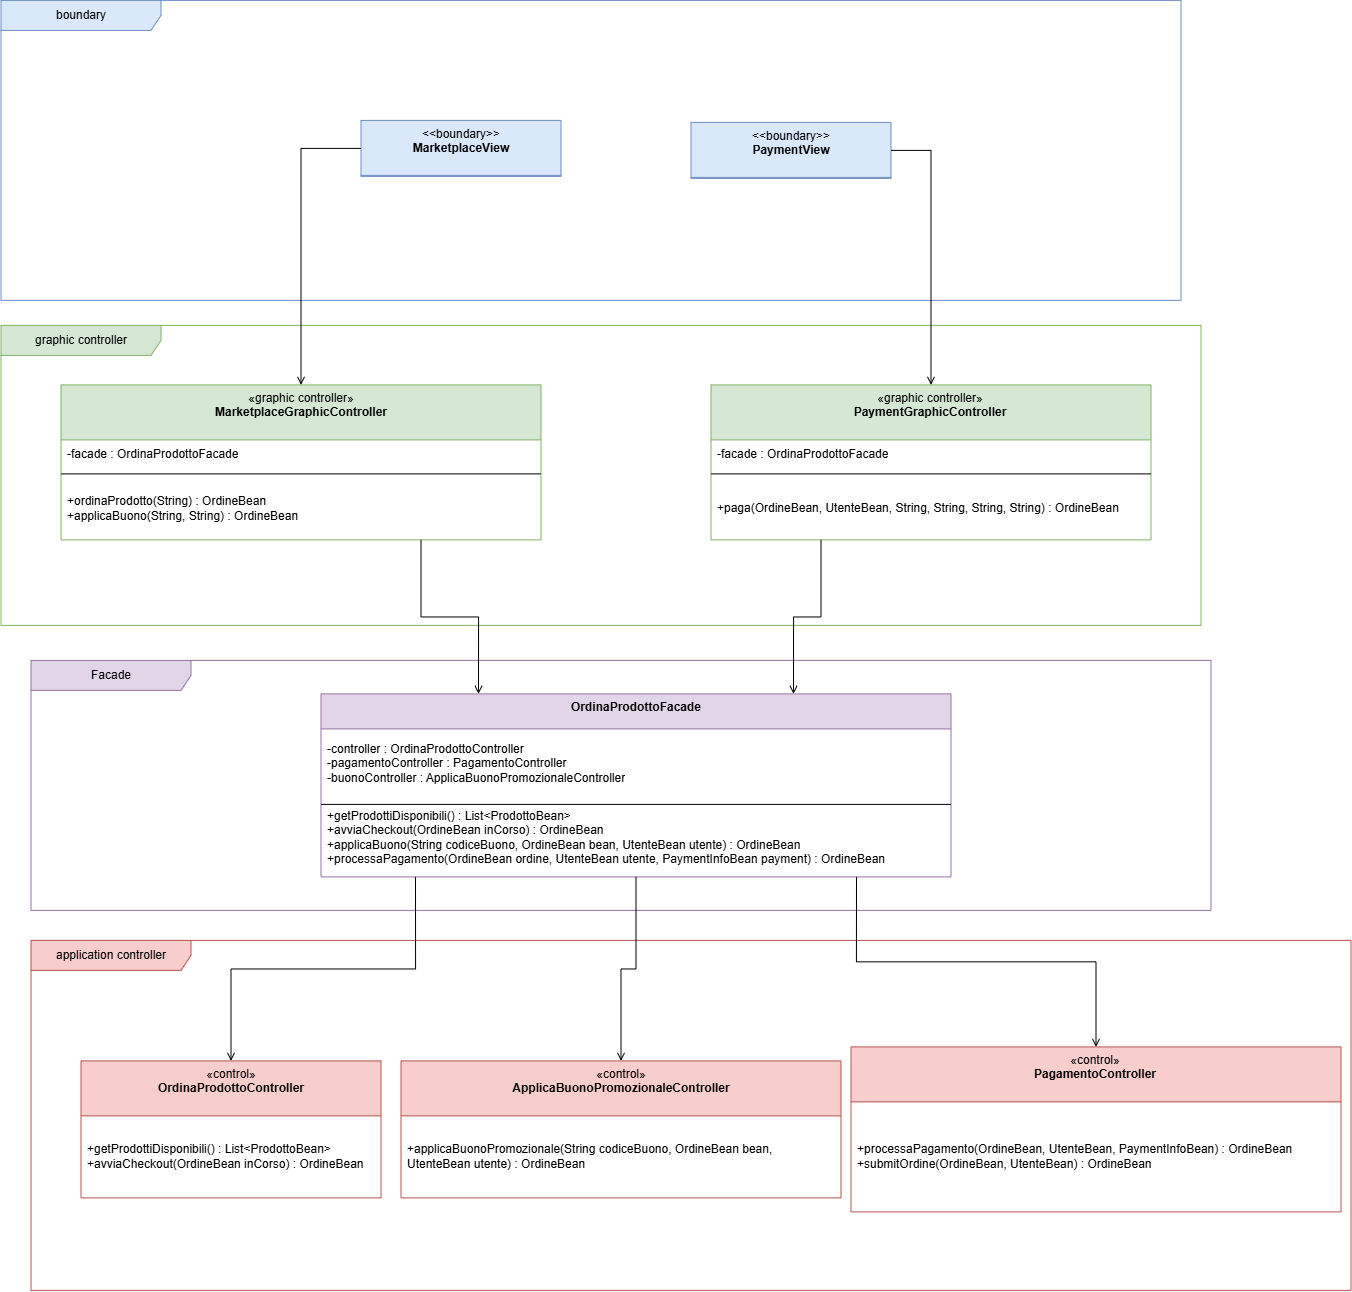
\includegraphics[width=0.75\textwidth]{figures/dl_facade_hr.png}
    \caption{Facade of the UC-04 checkout.}
    \label{fig:dl_facade}
\end{figure}
\texttt{OrdinaProdottoFacade} exposes to the graphic controller a single
interface for the checkout (\texttt{getProdottiDisponibili},
\texttt{avviaCheckout}, \texttt{applicaBuono}, \texttt{processaPagamento})
and hides the business subsystem, formed by the base controller and by the
extension controllers (voucher 4a and payment 6/6a). The client (boundary or
graphic controller) does not know the order in which the methods of the
application controllers are called. The operations of the extensions (
\texttt{applicaBuono}, \texttt{processaPagamento}) live only in their
respective sub-controllers: the Facade invokes them directly and the base
controller does not re-expose them (no useless pass-through / indirection).

\section{Activity Diagram}
\label{sec:comportamentale}

\begin{figure}[H]
    \centering
    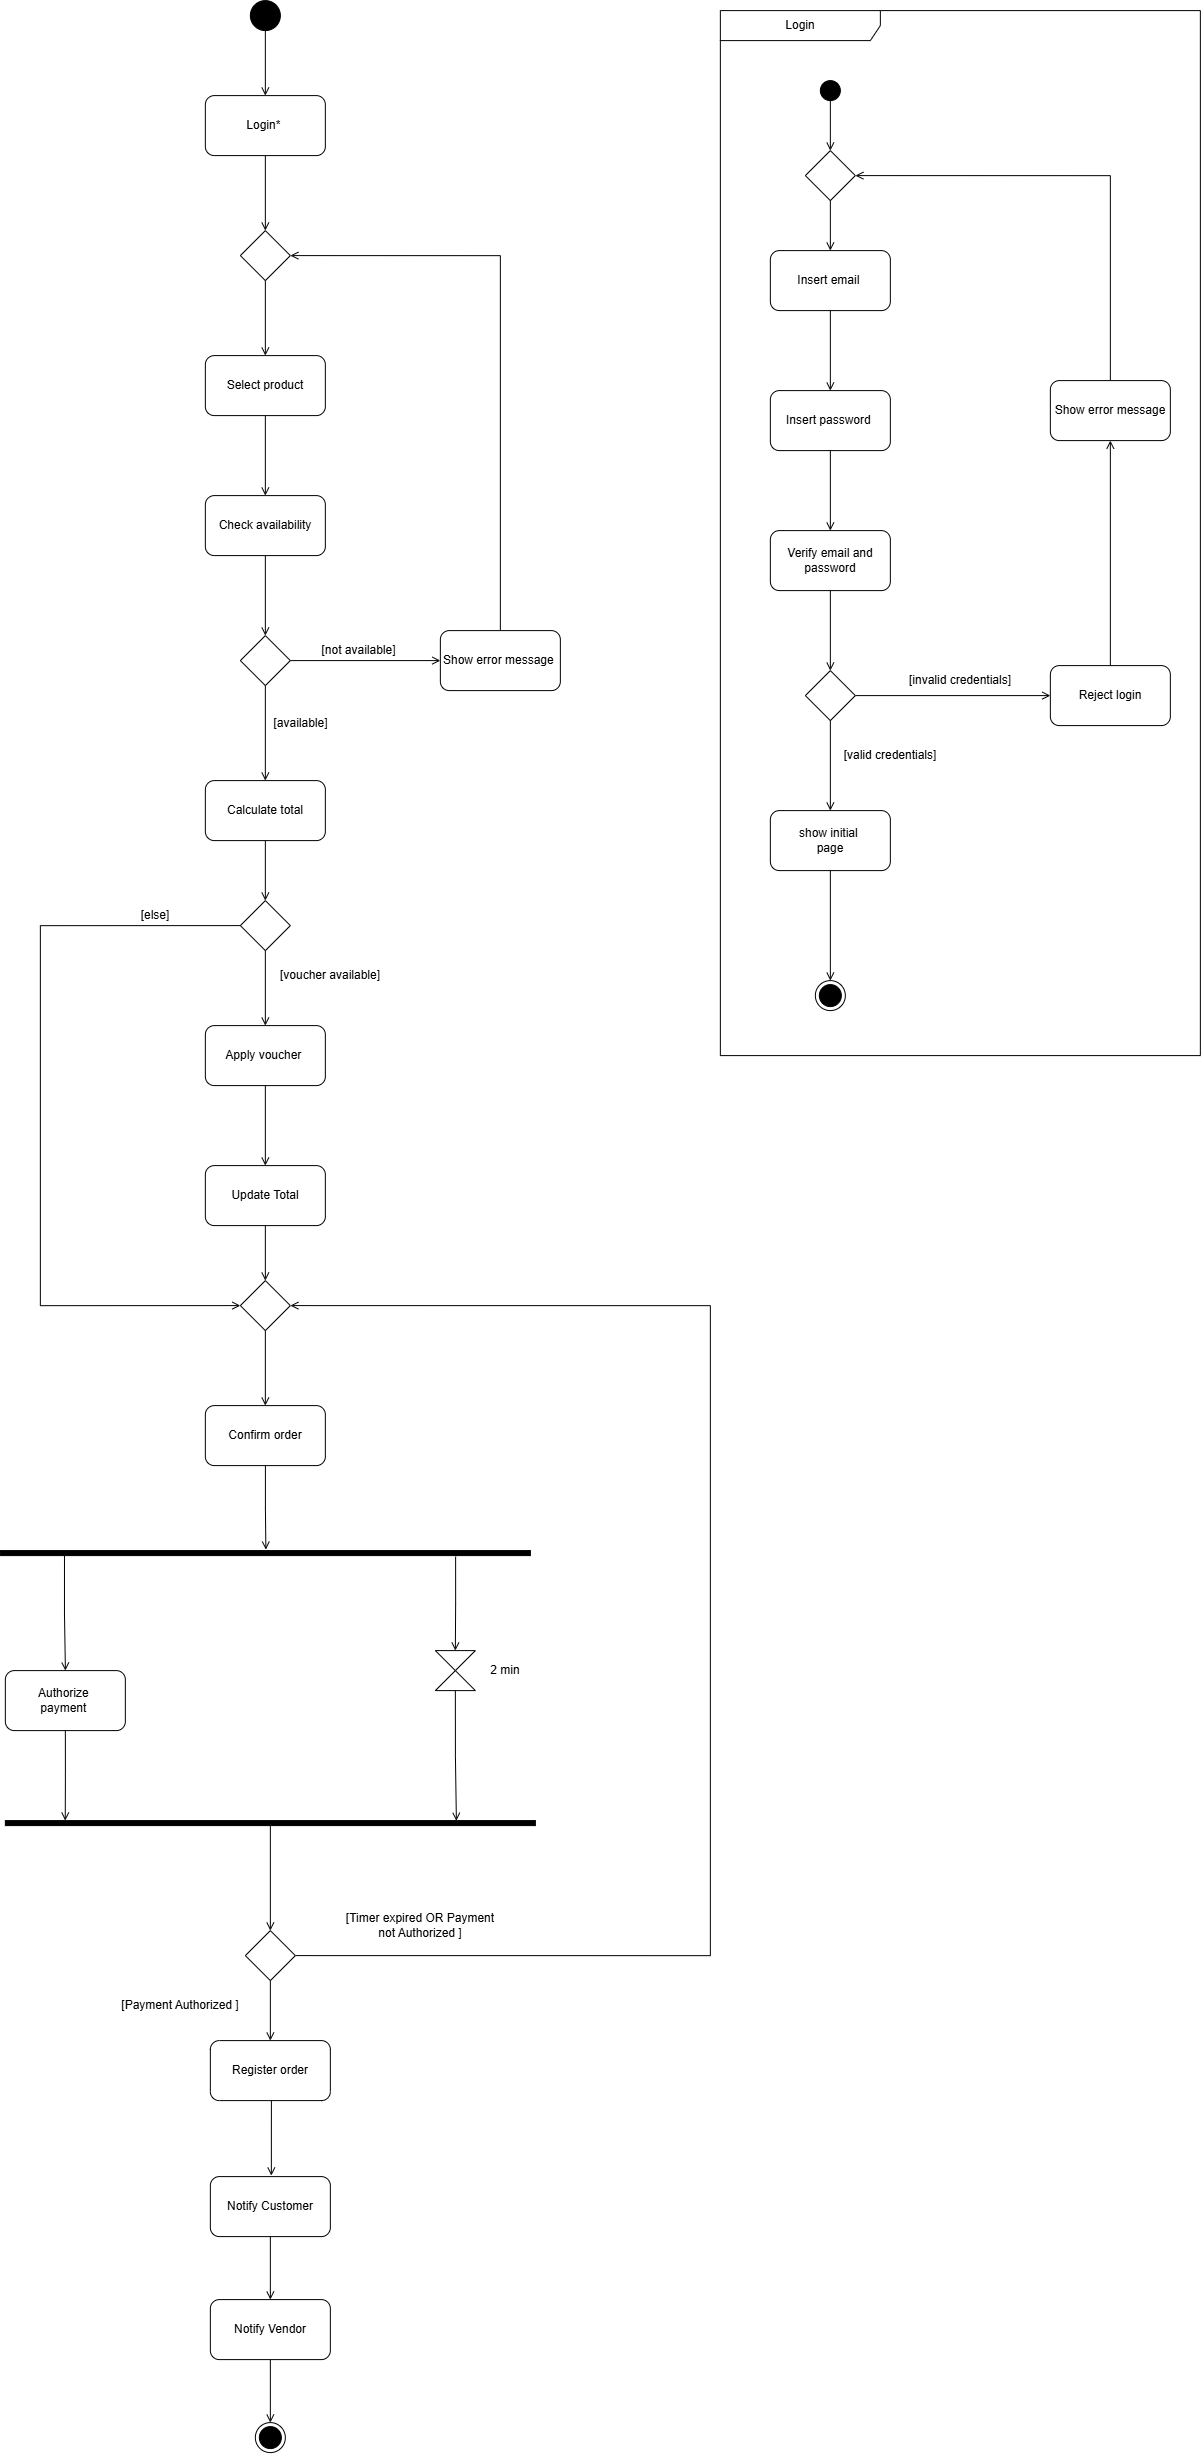
\includegraphics[height=0.8\textheight]{figures/activity_uc04.png}
    \caption{Activity diagram of UC-04: availability check, voucher application,
    payment authorization and sequential notification to buyer and vendor.}
    \label{fig:activity}
\end{figure}

\section{Sequence Diagram}
\label{sec:sequence}

\begin{figure}[H]
    \centering
    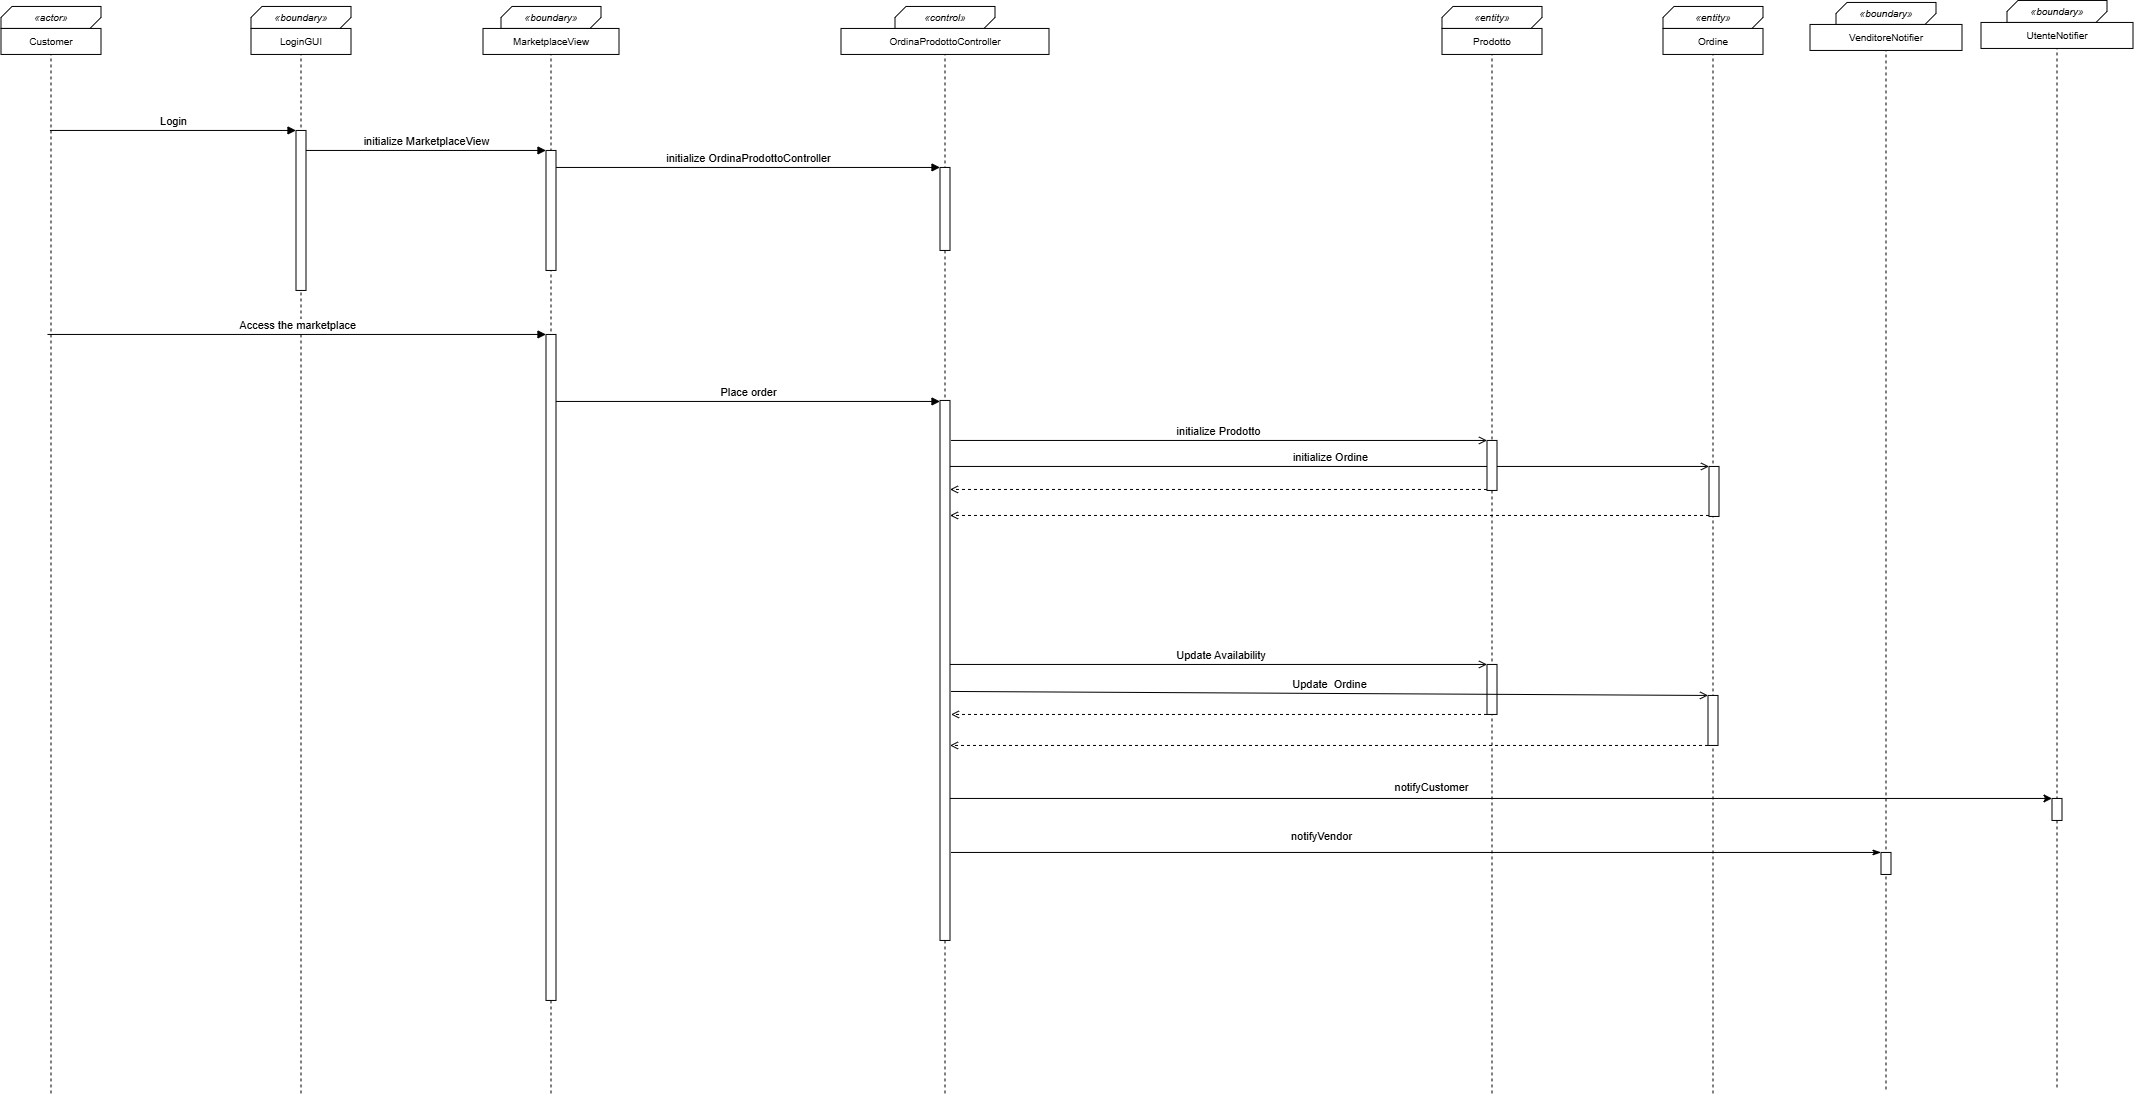
\includegraphics[width=\textwidth]{figures/seq_uc04_clean.png}
    \caption{Sequence diagram of UC-04.}
    \label{fig:sequence}
\end{figure}

\section{State Diagram}
\label{sec:state}

\begin{figure}[H]
    \centering
    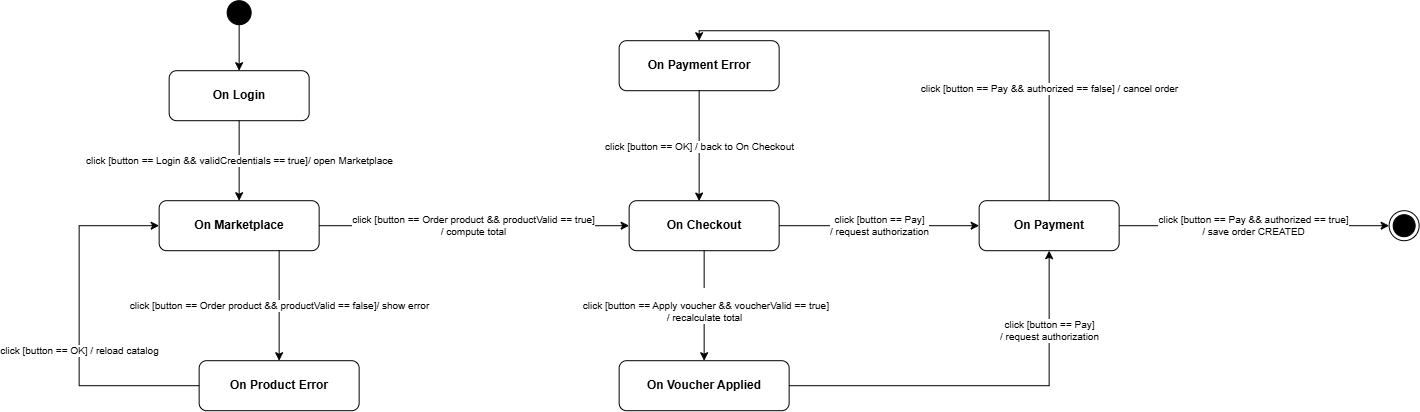
\includegraphics[width=\textwidth]{figures/state_uc04.png}
    \caption{State diagram of UC-04 Order a Product: navigation and alternative flows \texttt{3a}, \texttt{4a} and \texttt{6a}.}
    \label{fig:state}
\end{figure}


% CHAPTER 4 — TESTING
\chapter{Testing}
\label{cap:testing}

The verification of the system is carried out with a \textbf{JUnit 5} unit
test suite run by Maven, with coverage measured by JaCoCo (quality gate on
line coverage). The verified behaviors are described below, grouped by feature.

\paragraph{Access to the restricted area.} We tested the controller of the
restricted area by verifying that an authenticated user correctly retrieves
the data of their checkout and their session. The tests guarantee that the
returned structures are never \texttt{null} and that the access to the
restricted data is handled correctly for authenticated users.

\paragraph{Order creation and submission.} We tested the ordering flow by
verifying that a product is selected and that the order is created with the
correct vendor. The tests guarantee that an order with a null user or product
is rejected and that the stock availability is reduced at purchase time
without negative stock.

\paragraph{Voucher discount (Strategy).} We tested the discount logic by
verifying that a valid voucher is applied to the order total. The tests
guarantee that empty, expired or invalid codes are rejected without
unhandled exceptions and that the discount calculation never produces
inconsistent amounts.

\paragraph{Payment and authorization.} We tested the payment subsystem by
verifying both the authorized and the rejected branch. The tests guarantee
that a rejected payment raises the correct application exception leaving the
order unchanged, and that invalid card data (CVV, non-positive amount,
missing order) are blocked without \texttt{NullPointerException}.

\paragraph{Authentication.} We tested the authentication mechanism by
verifying both valid and invalid credentials. The tests guarantee that a
correct login populates the session and that wrong email or password are
rejected, with the \texttt{logout} correctly clearing the session.

\paragraph{Order lifecycle (BR-04 state machine).} We tested the order state
machine by verifying the sequence \texttt{CREATED
$\rightarrow$ CONFIRMED $\rightarrow$ IN\_DELIVERY $\rightarrow$ DELIVERED}.
The tests guarantee that an illegal transition is blocked by the invalid state
exception.

\paragraph{Observer notification.} We tested the Observer pattern by verifying
that the publisher notifies the registered observers when an order is
confirmed. The tests guarantee that the event (\texttt{OrdineEvent}) is
delivered to the observers through the read-only DTO, never the domain entity.

\paragraph{Persistence (Demo and File System).} We tested the persistence
layers by verifying the create-read-update cycle of users, products and
orders. The tests guarantee that the \emph{Demo} (in-memory) and
\emph{File System} persistence keep the data consistently, including the
retrieval of products by name.

% CHAPTER 5 — EXCEPTIONS
\chapter{Exceptions}
\label{cap:exceptions}

The error logic is a taxonomy (\texttt{exception/}) that is fully
\textbf{checked}, forcing the explicit handling (\texttt{throws} /
\texttt{try/catch}).

\begin{center}
\begin{tabular}{@{}ll@{}}
\toprule
\textbf{Exception} & \textbf{Role} \\
\midrule
\texttt{CiboAmicoException} (abstract) & Checked base, common fields \\
\texttt{BusinessValidationException} & Violated business rule \\
\quad\texttt{AutenticazioneException} & Wrong credentials \\
\quad\texttt{InvalidStateTransitionException} & Illegal state (BR-04) \\
\texttt{DAOException} & Persistence (file / DB) \\
\bottomrule
\end{tabular}
\end{center}

The base \texttt{CiboAmicoException} extends \texttt{java.lang.Exception}
(\textbf{checked}) and exposes four fields: \texttt{userMessage} (shown to the
user), \texttt{technicalMessage} (for logs), \texttt{errorCode} and
\texttt{timestamp}. The views read only \texttt{getUserMessage()}.

\section{Wrapping}
\label{sec:exc_wrapping}

The DAOs wrap the low-level error (\texttt{SQLException},
\texttt{IOException}) in a \texttt{DAOException} with
\texttt{(message, cause)}: \texttt{getCause()} preserves the original cause,
which never propagates to the boundaries.

\section{Payment}
\label{sec:exc_payment}

\texttt{PaymentRejectedException} (\texttt{pattern.payment}) is checked:
an unauthorized transaction, handled by extension \texttt{6a} of UC-04.

\section{Messages}
\label{sec:exc_messaggi}

Texts are centralized in \texttt{ExceptionMessagesEnum} (logs) and
\texttt{UserErrorMessagesEnum} (user), without duplicated strings at the
throw points.

% CHAPTER 6 — PERSISTENCY
\chapter{Persistency}
\label{cap:persistenza}

Persistence is interchangeable at runtime (NFR-01): three mutually exclusive
backends are selected through the \textbf{Abstract Factory} pattern
(\texttt{DAOFactory} plus one concrete factory per mode).

\section{DB persistence layer (MySQL/JDBC)}
The DB persistence layer uses \textbf{MySQL} as a relational DBMS. Data
management is delegated to specific DAO classes (e.g.
\texttt{JDBCUserDAO}, \texttt{JDBCOrdineDAO}), which run SQL queries for the
CRUD operations on the entities.

\textbf{Main entities:}
\begin{itemize}
    \item \textbf{Users}: registered, with their roles (Customer and Vendor);
    \item \textbf{Orders}: transactional records with state, total and items;
    \item \textbf{Products}: marketplace items (catalog and inventory);
    \item \textbf{Vouchers}: discount codes (percentage or fixed amount).
\end{itemize}

Transactions are atomic (\texttt{ConnectionManager} uses
\texttt{setAutoCommit(false)} with \texttt{commit/rollback} for the stock
reduction).

\textbf{Configuration}: the system is configured through the
\texttt{config.properties} file by setting \texttt{persistence\_type = JDBC} and
providing the required MySQL credentials.

\section{FS persistence layer (File System)}
The FS persistence layer stores the data on \textbf{JSON} files in the
\texttt{data/} folder. Each entity is mapped to a dedicated file
(e.g. \texttt{utenti.json}, \texttt{ordini.json}, \texttt{prodotti.json},
\texttt{inventario.json}).

\textbf{Management}: the \texttt{GsonConfig} class provides a consistent JSON
serializer (helper for \texttt{LocalDate}/\texttt{LocalDateTime}) used by all
the FS DAOs to guarantee the correct reading/writing of the records.

\textbf{Configuration}: the mode is activated by setting
\texttt{persistence\_type = FS} in the configuration file.

\section{DEMO persistence layer (In-Memory)}
The DEMO persistence layer keeps the data exclusively in the volatile memory
(RAM), without permanent storage. The structures are populated with default
values at startup and cleared at the end of the execution.

\textbf{Use cases}: it is designed for unit testing, rapid development and
demonstrations that require no database configuration.

\textbf{Configuration}: the mode is activated by setting
\texttt{persistence\_type = DEMO} (default).

% CHAPTER 8 — LINKS
\chapter{Video and Links}
\label{cap:links}

\section{GitHub Repository}
\url{https://github.com/Damiano-o/ciboamico.git}

\section{SonarCloud}
\url{https://sonarcloud.io/organizations/ciboamico-ispw}

\section{Demonstration video}
\emph{To be added before the submission.}


\end{document}
